\documentclass{article}
\renewcommand*\familydefault{\sfdefault}
\usepackage[utf8]{inputenc}
\usepackage[T1]{fontenc}
\setlength{\textwidth}{481pt}
\setlength{\textheight}{650pt}
\setlength{\headsep}{10pt}
\usepackage{amsfonts}
\usepackage[T1]{fontenc}
\usepackage{palatino}
\usepackage{calrsfs}
\usepackage{geometry}
\geometry{ left=3cm, top=2cm, bottom=2cm, right=2cm}
\usepackage{xcolor}
\usepackage{amsmath}
\usepackage{tikz,tkz-tab}
\usepackage{cancel}
\usepackage{pgfplots}
\usepackage{pstricks-add}
\usepackage{pst-eucl}
\begin{document}
\title{Démonstration kholle 5}
\date{}
\maketitle
	\renewcommand{\thesection}{\Roman{section}}
	\setlength{\parindent}{1.5cm}
	\section{Exponentielle propriété et unicité}
	\textcolor{green}{Propriété :} \\
	On admet l'existence d'une fonction $f \in \mathcal{D}^1(\mathbb{R})$ tel que $f(0)=1$ et $f'=f$ \\
	Elle est unique. On la note exp (fonction exponentielle). \\
	De plus : \\
	$\forall x \in \mathbb{R}, (exp(x) \neq 0$ et $\frac{1}{exp(x)} = exp(-x))$ \\
	\textcolor{red}{Démonstration :} \\ 
	Soit f convenant, $f \in \mathcal{D}^1(\mathbb{R}), f(0)=1$ et $f'=f$ \\
	\indent \textcolor{red}{a)} $u:\mathbb{R} \rightarrow \mathbb{R}$ \\
	\indent $x \rightarrow f(x)f(-x)$ \\
	Alors $u \in \mathcal{D}^1(\mathbb{R})$ et pour $x \in \mathbb{R}$ \\
	$u'(x)=f'(x)f(-x)+f(x)(-f'(-x))$ \\
	or $f'=f$ donc : \\
	$\forall x \in \mathbb{R}, u'(x)=f(x)f(-x)-f(x)f(-x)=0$ \\
	u' est nulle sur l'intervalle $\mathbb{R}$ donc u est constante \\
	$\forall x \in \mathbb{R}, u(x)=u(0)=1$ car $f(0)=1$ \\
	$\forall x \in \mathbb{R}, \underbrace{f(x)}_{\neq 0, \quad inverse \quad de \quad f(-x)} f(-x) =1$ \\
	\textcolor{red}{b)} Si g convient aussi : \\
	Posons v : $\mathbb{R} \rightarrow \mathbb{R}$ \\
	\indent $x \rightarrow g(x)f(-x)$ \\
	alors $v \in \mathcal{D}^1(\mathbb{R})$ est pour $x \in \mathbb{R}$ : \\
	$v'(x)=g'(x)f(-x)+g(x)(-f'(-x))$ \\
	or $f'=f$ et $g'=g$ donc : \\
	$\forall x \in \mathbb{R}, v'(x)=g(x)f(-x)-g(x)f(-x)=0$ \\
	v' est nulle sur l'intervalle $\mathbb{R}$ donc v est constante \\
	$\forall x \in \mathbb{R}, v(x) =v(0)=1$ car $f(0)=g(0)=1$ \\
	$\forall x \in \mathbb{R}, g(x)f(-x)=1$ \\
	donc : \\
	$\forall x \in \mathbb{R}, g(x)\underbrace{f(-x)f(x)}_{=1 \quad par \quad a} =f(x)$ \\
	$g=f$ \\
	\section{exponentielle: strictement positive, croissante, limites, logarithme}
		\textcolor{green}{Propriété :} la fonction exponentielle est : \\
	\textcolor{green}{1)} strictement positive \\
	\textcolor{green}{2)} strictement croissante \\
	\textcolor{green}{3)} $\lim_{x \rightarrow + \infty} exp(x)=+ \infty,$ \\
	\textcolor{green}{4)} $\lim_{x \rightarrow - \infty} exp(x) =0$ \\
	\textcolor{red}{Démonstration :} \\
	\textcolor{green}{1)} exp ne s'annule pas (propriété précédente) et est continue sur l'intervalle $\mathbb{R}$. \\
	Elle ne change pas de signe (contraposé du TVI) $exp(0)=1>0$, son signe est donc $>0$ \\
	\textcolor{green}{2)} $exp'(0)= exp>0$ donc exponentielle strictement croissante sur l'intervalle $ \mathbb{R}$ \\
	\textcolor{green}{3)} Posons $f : \mathbb{R} \rightarrow \mathbb{R}$ \\
	$x \rightarrow exp(x)-(x+1)$ \\
	$f \in \mathcal{D}^1(\mathbb{R})$ et : \\
	\indent $\forall x \in \mathbb{R}, f'(x)= exp(x)-1$ >0 si x>0;\quad 0 si x=0;  \quad  <0 si x<0 \\
	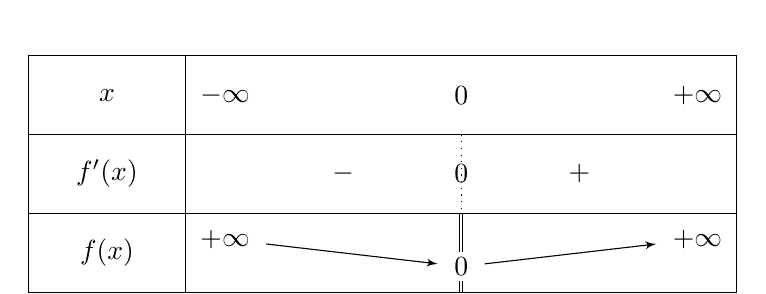
\begin{tikzpicture}
\tkzTabInit{$x$ / 1 , $f'(x)$ / 1, $f(x)$ / 1 }{$-\infty$, $0$, $+\infty$}
\tkzTabLine{, -, z, +,} 
 \tkzTabVar{+/ $+\infty$,  -C/ $0$, +/ $+\infty$,}
\end{tikzpicture}
\\
	D'après le tableau de variation $\forall x \in \mathbb{R},f(x)\geq0$ \\
	c'est-à-dire : $\forall x \in \mathbb{R}, exp(x) \geq x+1$ \\
	or $\lim_{x \rightarrow + \infty}(x+1)= +\infty$ \\
	donc $\lim_{x \rightarrow + \infty}(exp(x))= + \infty$ \\
	\textcolor{green}{4)} Ainsi $\lim_{x \rightarrow - \infty} \underbrace{(exp(-x))}_{\frac{1}{exp(x)}}=+\infty$ \\
	Donc $\lim_{x \rightarrow - \infty}(exp(x))=0$ \\
	{\bf Corolaire :} exp réalise une bijection de $\mathbb{R}$ dans $\mathbb{R}^*_+$. \\
	La réciproque est notéé ln (logarithme népérien). \\
	On a : $\lim_{x \rightarrow 0} \ln(x)= - \infty $ \\
	\indent $ \lim_{x \rightarrow + \infty} \ln(x)=+ \infty $ \\
	On pose $e=exp(1) \approx 2.718$ \\
	(On a donc $\ln(e)=1$, $\ln(1)=0$) \\
	\textcolor{red}{Démonstration : } corolaire du TVI appliqué à exp grâce à la  propriété précédente
	\section{Exponentielle de somme, logarithme de produit, dérivée de ln}
	\textcolor{green}{Propriété : }\\
	\textcolor{green}{1)} $\forall(a,b) \in \mathbb{R}^2,exp(a+b)=exp(a)exp(b)$ \\
	\textcolor{green}{2)} $\forall(a,b \in \mathbb{R}^2, exp(a-b)=\frac{exp(a)}{exp(b)}$ \\
	\textcolor{red}{Démonstration :} \\ \textcolor{green}{1)} Soit $a \in \mathbb{R}$ \\
Posons $f : \mathbb{R} \rightarrow \mathbb{R}$ \\
\indent $x \rightarrow exp(a+x)exp(-x)$ \\
$f \in \mathcal{D}^1(\mathbb{R})$ et :\\
\indent $\forall x \in \mathbb{R}, f'(x)=1exp'(a+x)exp(-x)	+ exp(a+x) (-exp'(-x))$ \\
Comme $exp'=exp$ : \\
\indent $f'(x)=0$ \\
f' est nulle sur $\mathbb{R}$ donc f est constante : \\
$\forall x \in \mathbb{R}, f(x)=f(0)=exp(a)$ car $exp(0)=1$ \\
$\forall x \in \mathbb{R}, exp(a+x) \underbrace{exp(-x)exp(x)}_{1} = exp(a)exp(x)$ \\
\textcolor{green}{2)} Soit $(a,b) \in \mathbb{R}^2$ \\
$exp(a)=exp(a-b+b)$ \\
Par \textcolor{green}{1} : \\
 $exp(a)=exp(a-b) \underbrace{exp(b)}_{\neq 0}$ \\
 $exp(a-b)=\frac{exp(a)}{exp(b)}$ \\
 \textcolor{green}{Propriété :} \\
 \textcolor{green}{1)}$\forall (a,b) \in (\mathbb{R}^*_+)^2, \ln(ab)=\ln(a) + \ln(b) $ \\
 \textcolor{green}{2)} $\forall (a,b) \in (\mathbb{R}^*_+)^2, \ln(\frac{a}{b})= \ln(a)-\ln(b)$ \\
 \textcolor{red}{Démonstration :} \\
 \textcolor{green}{1)} $exp(\ln(a)+\ln(b))= exp(\ln(a))exp(\ln(b))$ \\
 \indent $= a \times b$ \\
 \indent $= ab$ \\
 donc : \\
 $\ln (a) + \ln(b) = \ln(ab) $ \\
 \textcolor{green}{2)} $\ln(a)=\ln(\frac{a}{b}b)$ \\
 Par \textcolor{green}{1} : \\
 $\ln(a) = \ln(\frac{a}{b})+\ln(b)$ \\
 $\ln(\frac{a}{b})= \ln(a)-\ln(b)$ \\
 \textcolor{green}{Propriété :} \\
 $\ln \in \mathcal{D}^1(\mathbb{R}^*_+)$ et : \\
 \indent $\forall x \in \mathbb{R}^*_+,\ln'(x)=\frac{1}{x}$ \\
 \textcolor{red}{Démonstration :} exp' ne s'annule pas (car exp'=exp) donc ln est dérivable. \\
 \indent Soit $x \in \mathbb{R}^*_+$ et $y=\ln(x) \in \mathbb{R}$: \\
 $\ln'(x)=\frac{1}{exp'(y)}=\frac{1}{exp(\ln(x))}=\frac{1}{x}$
 \section{Croissances comparées  logarithme}
 \textcolor{green}{Propriété :} \\
 \textcolor{green}{1)} $\lim_{x \rightarrow + \infty} \frac{\ln(x)}{x}=0$ \\
 Soit $\alpha \in \mathbb{R}^*_+$ : \\
 \textcolor{green}{2)} $\lim_{x \rightarrow + \infty} \frac{\ln(x)}{x^\alpha}=0$ \\
 \textcolor{green}{3)}$\lim_{x \rightarrow 0} x^\alpha \ln(x) =0$ \\
 \textcolor{red}{Démonstration :} \\
 \textcolor{green}{1)} Soit $f :[1;+\infty [ \rightarrow \mathbb{R}$ \\
 \indent $x \rightarrow \ln(x)-2\sqrt{x}$ \\
 $\forall x \in [1;+\infty[, f'(x)=\frac{1}{x}-\frac{1}{\sqrt{x}},$ =0 si x=1, <0 si x>1 \\
 donc f est strictement décroissante sur $[1,+\infty[$ \\
 donc $\forall x \in [1; +\infty[,f(x)\leq f(1)=-2 \leq 0$ \\
 Comme $x\geq 1$ et $f \leq 0$ : \\
 $\forall x \in [1;+ \infty[, 0 \leq \ln(x) \leq 2 \sqrt{x}$
 puis: \\
 $\forall x \in [1 ; +\infty [,0 \leq \frac{\ln(x)}{x} \leq \frac{2}{\sqrt{x}}$ \\
 or $\lim_{x \rightarrow + \infty} \frac{2}{\sqrt{x}}=0$ \\
 donc $\lim_{x \rightarrow + \infty} \frac{\ln(x)}{x}=0$ \\
 \textcolor{green}{2)} On a : $\lim_{x \rightarrow +\infty} \frac{\ln(x)}{x}=0$ \\
 et $\lim_{x \rightarrow +\infty} x^\alpha = +\infty$ car $\alpha > 0$ \\
 donc : $\lim_{x \rightarrow + \infty} \frac{\ln(x^\alpha)}{x^\alpha}=0$ \\
 $\lim_{x \rightarrow + \infty} \alpha \frac{\ln(x)}{x^\alpha}=0$ \\
 or $ \alpha \neq 0$ donc \\
 $\lim_{x \rightarrow +\infty} \frac{\ln(x)}{x^\alpha}=0$ \\
 \textcolor{green}{3)} par \textcolor{green}{2} $\lim_{x \rightarrow + \infty} \frac{\ln(x)}{x^\alpha}=0$ \\
 $\lim_{x \rightarrow 0^+} \frac{1}{x}=+ \infty$ \\
 donc $\lim_{x \rightarrow 0^+}\frac{\ln(1/x)}{1/x^\alpha}=0$ \\
 $\lim_{x \rightarrow 0^+} x^\alpha \ln(x) =0$ \\
 Comme ln(x) n'est pas défini sur x<0  on a : \\
 $\lim_{x \rightarrow 0} x^\alpha \ln(x) =0$
 \section{Croissances comparées exponentielle}
 \textcolor{green}{Propriété :} \\
 \textcolor{green}{1)} $\lim_{x \rightarrow + \infty} \frac{e^x}{x}= +\infty$ \\
 Soit $\alpha \in \mathbb{R}^*_+$ : \\
 \textcolor{green}{2)} $\lim_{x \rightarrow + \infty} \frac{e^x}{x^\alpha}= +\infty$ \\
 \textcolor{green}{3)}$\lim_{x \rightarrow - \infty} x^n e^x=0$ \\
 \textcolor{red}{Démonstration :} \\
 \textcolor{green}{1)} On a : \\
 $\lim_{x \rightarrow + \infty} \frac{\ln(x)}{x}=0$ \\
 et $\lim_{x \rightarrow + \infty}e^x=+\infty$ \\
 donc $\lim_{x \rightarrow + \infty} \frac{\ln(e^x)}{e^x}=0$ \\
 $\lim_{x \rightarrow + \infty} \frac{x}{e^x}=0$ strictement positif pour x>0 \\
 donc : \\
 $\lim_{x \rightarrow + \infty} \frac{e^x}{x}= +\infty$ \\
 \textcolor{green}{2)} Cas général avec $\alpha > 0$ : \\
 $\lim_{x \rightarrow + \infty} \frac{e^x}{x}= + \infty$ (par \textcolor{green}{1}) \\
 et $\lim_{x \rightarrow + \infty}\frac{x}{\alpha}= + \infty$ car $\alpha > 0$ \\
 donc $\lim_{x \rightarrow + \infty} \frac{e^{x/\alpha}}{x /\alpha}=+ \infty$ \\
 $\lim_{x \rightarrow + \infty} \cancel{\alpha} \frac{e^{x/\alpha}}{x}= + \infty$ car $\alpha>0$ \\
 enfin : $ \lim_{x \rightarrow + \infty} x^\alpha= +\infty$ car $\alpha>0$ \\
 donc $\lim_{x \rightarrow + \infty}(\frac{e^{x/\alpha}}{x})^\alpha = + \infty$ \\
 \indent $= \frac{e^x}{x^\alpha}$ \\
 \textcolor{green}{3)} $n \in \mathbb{N}^*$ donc par \textcolor{green}{2} : \\
 $\lim_{x \rightarrow + \infty }\frac{e^x}{x^n}=+ \infty$ \\
 or $\lim_{x \rightarrow - \infty} (-x) = + \infty$ \\
 donc \\
 $\lim_{x \rightarrow - \infty} \frac{e^{-x}}{(-x)^n}=+ \infty$ \\
 $ \lim_{x \rightarrow - \infty} \frac{1}{(-1)^nx^ne^x}= + \infty$ \\
 $ \lim_{x \rightarrow - \infty} \underbrace{\cancel{(-1)^n}}_{constante \quad \neq 0} x^ne^x=0$
	\section{Fonction arcsin : dérivation justification de $\cos(arcsin(x))= \sqrt{1-x^2}$, tracé avec sinus}
	\textcolor{green}{Propriété :} \\
	\textcolor{green}{1)} $ \forall x \in [-1;1],\sin(\arccos(x))=cos(arcsin(x))=\sqrt{1-x^2}$ \\ 
	\textcolor{green}{2)}arcsin est dérivable sur  ]-1;1[ : \\
	$\forall x \in ]-1;1[,\quad arcsin'(x)=\frac{1}{\sqrt{1-x^2}}$ \\
	\textcolor{red}{Démonstration :} \\ 
	\textcolor{green}{1)} Posons $\theta = \arccos(x)$ et $y=sin(\theta)$ \\
	On a $\cos(\theta)=x$ et $0 \leq \theta \leq \pi$ \\
	On sait que : \\
	$\sin^2(\theta) + \cos^2(\theta)=1$ \\
	c'est-à-dire $y^2 + x^2= 1$ \\
	\indent $y^2=1-x^2$ \\
	Or $y= \sin(\theta)$ avec $0 \leq \theta \leq \pi$ \\
	donc $y \geq 0$ \\
	donc $y= \sqrt{1-x^2}$ \\
	c'est-à-dire : $\sin(\arccos(x))= \sqrt{1-x^2}$ \\
	Puis : \\
	$\cos(\arcsin(x))=cos(\frac{\pi}{2}-\arccos(x))$ \\
	\indent $=\sin(\arccos(x))$ \\
	\textcolor{green}{2)} La fonction : \\
	 $f : [-\frac{\pi}{2}; \frac{\pi}{2}] \rightarrow \mathbb{R}$ \\
\indent $ x \rightarrow \sin(x) $ \\
Celle-ci est continue et strictement croissant sur $[- \frac{\pi}{2};\frac{\pi}{2}]$ \\
Elle réalise une bijection sur image [-1 ; 1] \\
Et par définition, $\arcsin=f^{-1}$ \\
Ainsi : \\
$arcsin \in \mathcal{C}^0([-1;1])$ et arcsin est dérivable en un point $x \in [-1 ; 1]$ \\
ssi $sin'(y) \neq 0$ où $y=\arcsin(x)$ \\
et dans ce cas : \\
 \indent $\arcsin'(x) = \frac{1}{\sin'(y)}$ \\
or : si $x= -1$, $y= \frac{\pi}{2}$ et  $sin'(y)=0$ car $sin'=cos$ \\
si $x=1$, $y= \frac{\pi}{2}$ et $\sin'(y)=0$ car $sin'=cos$ \\
si $-1<x<1$, $-\frac{\pi}{2}<y<\frac{\pi}{2}$ et $sin'(y)>0$ car $sin'=cos$ \\
Pour $ x \in ]-1;1[$ : \\
$\arcsin'(x)= \frac{1}{\sin'(\arcsin(x))}$ \\
\indent $=\frac{1}{\cos(\arcsin(x))}$ \\
\indent $=\frac{1}{\sqrt{1-x^2}}$ \\
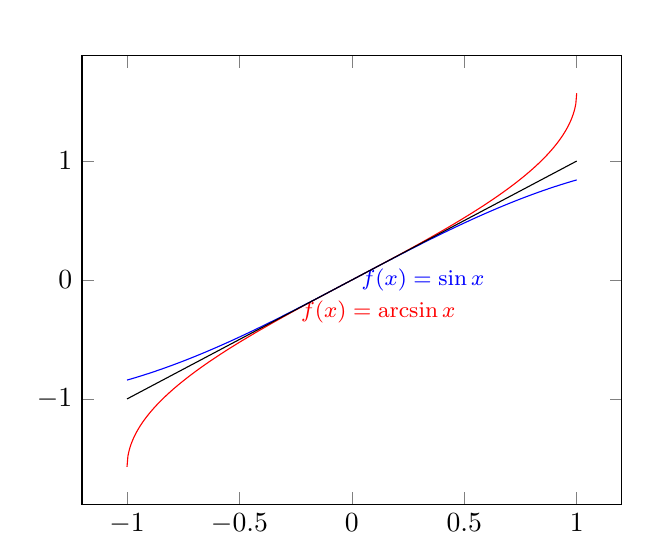
\begin{tikzpicture}
  \begin{axis}[domain = -1:1, samples = 500]
    \addplot[color = red]  {asin(x)/180*pi}
    node[right,pos=0.4,font=\footnotesize]{$f(x)=\arcsin  x$};
    \addplot[color = blue] {sin(deg(x))}
    node[right,pos=0.5,font=\footnotesize]{$f(x)=\sin  x$};;
    \addplot[color = black] {x};
      \end{axis}
\end{tikzpicture}
	\section{arccosinus: dérivation(avec $\arcsin(x) + \arccos(x) =\frac{\pi}{2}$) tracé avec le cosinus}
	\textcolor{green}{Propriété :} \\
	 \textcolor{green}{1)} $\forall x \in [-1 ; 1 ],\quad \arcsin(x) +arccos(x) = \frac{\pi}{2} $ \\
	 \textcolor{green}{2)} arccos est dérivable sur  ]-1;1[ : \\
	$\forall x \in ]-1;1[,\quad arccos'(x)=-\frac{1}{\sqrt{1-x^2}}$ \\
	\textcolor{red}{Démonstration :} \\
	\textcolor{green}{1)} Posons $ \theta = \arcsin(x)$ : $\sin(\theta)=x$ et $-\frac{\pi}{2}\leq \theta \leq \frac{\pi}{2}$ \\
	On a : \\
	$\cos(\frac{\pi}{2}-\theta)=sin(\theta)=x$ \\
	or : $ -\frac{\pi}{2} \leq - \theta \leq \frac{\pi}{2},$ donc $0 \leq \frac{\pi}{2}-\theta \leq \pi $ \\
	donc : $\frac{\pi}{2}- \theta = \arccos(x)$ \\
	Comme $\theta= \arcsin(x)$ \\
	$\frac{\pi}{2}-\arcsin(x)=\arccos(x)$ \\
	$\arccos(x) + \arcsin(x) =\frac{\pi}{2}$ \\
	\textcolor{green}{2)} Comme on a : \\
	$\arccos=\frac{\pi}{2}-\arcsin$ \\
	donc $\arccos'=-\arcsin'$ \\
	$\arccos' = - \frac{1}{\sqrt{1-x^2}}$ \\
	\begin{tikzpicture}
  \begin{axis}[domain=-1:1, samples=500, axis lines*=middle, xtick={-3.14,3.14}, ytick={-1.57,1.57}, yticklabels={$-\pi$/2,$\pi$/2},xticklabels={$-\pi$,$\pi$}]
    \addplot[color = red]  {acos(x)/180*pi}
    node[right,pos=0.4,font=\footnotesize]{$f(x)=\arccos  x$};
    \addplot[color = blue][domain = 0:3.14, samples = 500] {cos(deg(x))}
    node[right,pos=0.5,font=\footnotesize]{$f(x)=\cos  x$};;
    \addplot[color = black][domain = 0:3, samples = 500] {x};
      \end{axis}
\end{tikzpicture}
	\section{arctangente : dérivation (avec justification $tan'(x)= 1+ tan^2(x)$), tracé avec tangente }
	\textcolor{green}{Propriété :} \\
	 \textcolor{green}{1)} $\forall x \in \mathcal{D}_{tan}, \tan'(x)=1+\tan^2(x)= \frac{1}{\cos^2(x)}$  \\ 
	\textcolor{green}{2)} $\arctan \in \mathcal{D}^1(\mathbb{R})$ et : \\
	$\forall x \in \mathbb{R}, \quad \arctan'(x)=\frac{1}{1+x^2}$ \\
	\textcolor{red}{Démonstration :} \\
	\textcolor{green}{1)}	 $\tan'(x)= \frac{\sin'(x)\cos(x)-sin(x)cos'(x)}{\cos^2(x)}$ \\
	\indent $=\frac{\sin^2(x)+cos^2(x)}{\cos^2(x)} = \frac{1}{\cos^2(x)}$ ou $\frac{\sin^2(x)}{\cos^2(x)} + \frac{\cos^2(x)}{\cos^2(x)}= 1 + \tan^2(x)$ \\
	\textcolor{green}{2)} soit $f : ]-\frac{\pi}{2};\frac{\pi}{2}[ \rightarrow \mathbb{R}$ : \\
	\indent $x \rightarrow \tan(x)$ \\
	$f \in \mathcal{D}^1(]-\frac{\pi}{2};\frac{\pi}{2}[)$, strictement croissante, réalise une bijection sur $]-\frac{\pi}{2};\frac{\pi}{2}[$ dans $\mathbb{R}$ \\
	Comme f' ne s'annule pas sur $]-\frac{\pi}{2};\frac{\pi}{2}[$, $f^{-1}$ est dérivable sur $\mathbb{R}$ et : \\
	$\forall x \in \mathbb{R},(f^{-1})'(x)= \frac{1}{f'(f^{-1}(x))}$ \\
	or : $f'= 1+ f^2$ \\
	donc pour $x \in \mathbb{R}$ : \\
	$f'(f^{-1}(x))=1+(f(f^{-1}(x)))^2$ \\
	\indent $= 1+x^2$ \\
	On a donc : \\
	$\arctan'(x)=\frac{1}{1+x^2}$ \\
	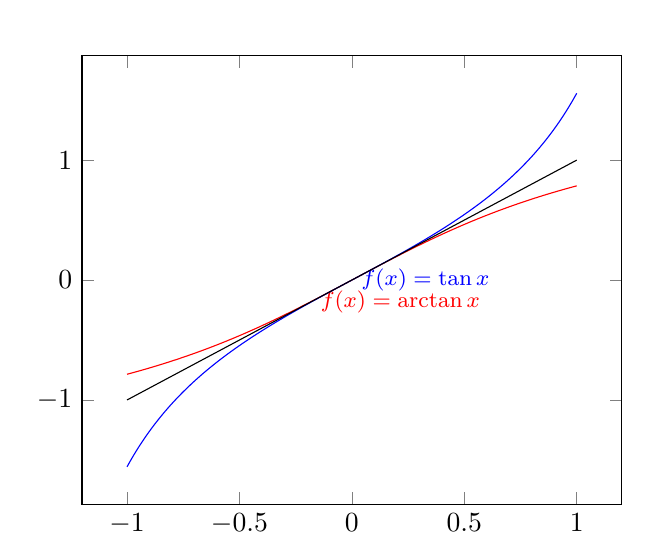
\begin{tikzpicture}
  \begin{axis}[domain = -1:1, samples = 500]
    \addplot[color = red]  {atan(x)/180*pi}
    node[right,pos=0.4,font=\footnotesize]{$f(x)=\arctan  x$};
    \addplot[color = blue] {tan(deg(x))}
    node[right,pos=0.5,font=\footnotesize]{$f(x)=\tan  x$};;
    \addplot[color = black] {x};
      \end{axis}
\end{tikzpicture}
	\section{\'Etude de $\arctan(x)+ \arctan (1/x)$ dérivation et trigonométrie}
	\textcolor{green}{Propriété :} \\
	$\forall x \in \mathbb{R}^*_+$, $\arctan(x)+ \arctan (1/x)=\frac{\pi}{2}$ \\
	$\forall x \in \mathbb{R}^*_-$, $\arctan(x)+ \arctan (1/x)=-\frac{\pi}{2}$ \\
	\textcolor{red}{Démonstration :} \\
	\textcolor{red}{Par dérivation :} \\
	Posons $f : \mathbb{R}^* \rightarrow \mathbb{R}$ \\
	\indent $x \rightarrow \arctan'(x) + \arctan(1/x)$ \\
	$f \in \mathcal{D}^1(\mathbb{R}^*)$ et : \\
	$\forall x \in \mathbb{R}^*, f'(x)=\frac{1}{1+x^2}+ \frac{1}{x^2} \frac{1}{1+(1+x)^2}=0$ \\
	f est constante sur chaque intervalle sur chaque intervalle : $\mathbb{R}^*_+$ et $\mathbb{R}^*_-$ \\
	Or : $f(1)= \frac{\pi}{2}$ \\
	$f(-1)=-\frac{\pi}{2}$ \\
	On a donc bien :
		$\forall x \in \mathbb{R}^*_+$, $f(x)=\frac{\pi}{2}$ \\
	$\forall x \in \mathbb{R}^*_-$, $f(x)=-\frac{\pi}{2}$  \\
	\textcolor{red}{Par trigonométrie :} \\
	Posons $ \theta = \arctan(x)$ \\
	$\tan(\theta) = x$ et $-\frac{\pi}{2}<\theta<\frac{\pi}{2}$
	$\theta \neq 0$ car $x \neq 0$ \\
	On a :
	$\tan(\frac{\pi}{2}- \theta ) = \frac{1}{\tan(\theta)}=\frac{1}{x}$ \\
	$- \frac{\pi}{2}<-\theta<\frac{\pi}{2}$ donc $0< \frac{\pi}{2}-\theta < \pi$ \\
	$1^{er}$ cas : $\theta > 0$ (c'est-à-dire x>0) \\
	\indent alors : $0< \frac{\pi}{2}-\theta< \frac{\pi}{2}$ \\
	donc $ \frac{\pi}{2}-\theta = \arctan(\frac{1}{x})$ \\
	On trouve: $ \frac{\pi}{2}-\arctan(x)= \arctan(\frac{1}{x})$ \\
	\indent $\arctan(\frac{1}{x}) +\arctan(x)=\frac{\pi}{2}$ \\
	$2^{eme}$ cas : $\theta < 0$ (c'est-à-dire x<0) \\
	alors $ \frac{\pi}{2}<\frac{\pi}{2}- \theta < \pi $ \\
	donc $- \frac{\pi}{2}<-\frac{\pi}{2}-\theta<0$ \\
	On a : $\tan(-\frac{\pi}{2}-\theta)= \tan(\frac{\pi}{2}-\theta)= \frac{1}{x}$ \\
		d'où : $-\frac{\pi}{2}-\theta= \arctan(\frac{1}{x})$ \\
		On trouve $ \theta - \theta -\frac{\pi}{2}=-\frac{\pi}{2}$
	\section{$x^x$, limite de la suite de terme général $(1+\frac{1}{n})^n$}
	\textcolor{red}{$x^x$ :} \\	
	Soit $f : \mathbb{R}^*_+ \rightarrow \mathbb{R}$ \\
	\indent $x \rightarrow x^x$ \\
	Il ne s'agit pas d'une fonction puissance car {\bf l'exposant est variable}.
	Revenons à la définition : \\
	\indent $f(x)=exp(x(\ln(x)))$ \\
	$f \in \mathcal{D}(\mathbb{R^*_+}$ car composition de fonction dérivable \\
	$\forall x \in \mathbb{R}^*_+,\quad f'(x)=(1+\ln(x))exp(x\ln(x))$ \\
		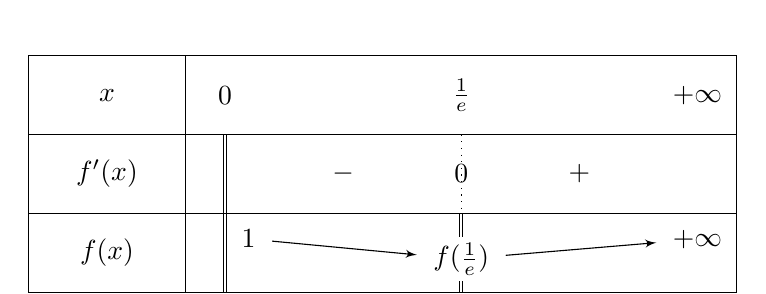
\begin{tikzpicture}
\tkzTabInit{$x$ / 1 , $f'(x)$ / 1, $f(x)$ / 1 }{$0$, $\frac{1}{e}$, $+\infty$}
\tkzTabLine{d, -, z, +,} 
 \tkzTabVar{D+/ $1$,  -C/ $f(\frac{1}{e})$, +/ $+\infty$,}
\end{tikzpicture}
\\
$\lim_{x \rightarrow 0} f(x)=1$ par croissance comparée \\ \\
\textcolor{red}{$1+\frac{1}{n}$} \\
$U_n=(1+\frac{1}{n})^n$ \\
$\ln(U_n)=n \ln(1 + \frac{1}{n})$ \\
$\ln(U_n)=\frac{\ln(1+1/n)}{1/n}$ \\
or : $\lim_{x \rightarrow 0} \frac{\ln(1+x)}{x}=1$ \\
et $\lim_{n \rightarrow + \infty} \frac{1}{n}=0 \quad \lim_{n \rightarrow +\infty} \ln(U_n)=1$ \\
On a donc $ \lim_{n \rightarrow + \infty}=exp(1)=e$ 
\end{document}
